%% LyX 2.0.3 created this file.  For more info, see http://www.lyx.org/.
%% Do not edit unless you really know what you are doing.
\documentclass{article}
\renewcommand{\sfdefault}{cmss}
\usepackage[utf8]{inputenc}
\usepackage{fancyhdr}
\pagestyle{fancy}
\usepackage{prettyref}
\usepackage{float}
\usepackage{rotfloat}
\usepackage{graphicx}
\usepackage[authoryear]{natbib}
\usepackage[unicode=true,pdfusetitle,
 bookmarks=true,bookmarksnumbered=false,bookmarksopen=false,
 breaklinks=false,pdfborder={0 0 1},backref=section,colorlinks=false]
 {hyperref}
\usepackage{breakurl}

\makeatletter

%%%%%%%%%%%%%%%%%%%%%%%%%%%%%% LyX specific LaTeX commands.
%% A simple dot to overcome graphicx limitations
\newcommand{\lyxdot}{.}


\makeatother

\begin{document}

\title{Planning Report - Running with Sound: Android Application Simulating
Sound Sources at GPS Coordinates Using Smartphone Sensors}


\author{Anton Palmqvist\\
880906-4010 \and Daniel Johansson\\
920815-4493 \and Joakim Johansson\\
921024-4530 \and Linus Karlsson\\
920731-2852 \and Marcus Bernhard\\
920125-1197}

\maketitle
Group 42

\tableofcontents{}


\section{Background}

The chosen subject, being combining a running application with guiding
sounds, is to our knowledge unusual. This makes the subject academically
interesting, since it is a new area to explore. Computer games make
use of sound to enhance the user experience, but with modern smartphone
sensors the same could be done in an outdoor environment to create
a virtual reality in sound.

There are currently multiple running applications making use of GPS
technology in order to measure speed and distance. Some, like “Zombies,
run!” even tracks the speed and simulates monsters approaching (audio)
if the user’s speed is too slow \citep{SixtoStart2014}. However,
the sound effects aren’t directional, meaning that the direction of
which the sound is not important for the game’s functionality - it
acts more like a cool feature.

By combining sound with the running game concept it would be possible
to hear something, for example a coin, and by running towards it be
able to obtain it when its location is reached. At the same time monsters
could be heard from a specific direction and by running in another
direction they could be avoided. These features will be a great motivator
for people struggling with motivation to workout on a regular basis.

Other academical parts that will not be mainly focused on but still
could be useful to have in mind is the behaviour science of what makes
a game fun and motivating. Therefore the target group of the application
is not only people who run regularly, but also people who need motivation
to do so.

Also it might be useful to investigate some shortest paths algorithms
for the running track.

All of this will be encapsulated in an Android application.


\section{Purpose}

The general purpose of the project is to make an application that:
\begin{enumerate}
\item Registers running activity and presents its statistics.
\item Uses the techniques of sound and sensors in a meaningful way.
\item Makes it enjoyable and motivating for people to exercise.
\end{enumerate}

\section{Problem/Assignment}


\subsection{Main goal}

The goal of the assignment is to create a fully functional running
game that is fun to use. To do this, the following milestones have
been created.
\begin{enumerate}
\item First of all the functions of a running app will be implemented. This
will include:

\begin{itemize}
\item GPS-positioning of the user.
\item The bearing of the user. (The user rotation relative to the compass
pointing north)
\item GPS-destinations that the user can run towards.
\item Statistics after a run.

\begin{itemize}
\item Time - The time you have been out running.
\item Distance - The total distance off your jogging.
\item Speed - Time per kilometer.
\item Altitude - Altitude-changes during the route.
\end{itemize}
\item Running High Scores.
\item Best time for given distances.
\end{itemize}
\item Secondly game functions will be implemented:

\begin{itemize}
\item Sound

\begin{itemize}
\item The sound will be directional, meaning that the sound will appear
to come from a specific direction of which the runner is supposed
to run towards - by balancing the audio level between the left and
right ear \citep{Roads1996}.
\item The level of the audio will change as the user is approaching or running
away from the GPS coordinate set as target.
\end{itemize}
\item Putting a monster on the map, which will be a moving destination.
Games with monsters might be:

\begin{itemize}
\item BETA - With the help of audio-navigation you have to run to a predefined
spot on the map.
\item Freerun - You can run anywhere you want without any special goals
while monsters are chasing you.
\item Quest - With the help of audio-navigation you have to run to a predefined
spot on the map while monsters are chasing you.
\item Under attack - You can run anywhere you want but the amount of monsters
that are chasing you are continuously growing and are becoming faster
until they catch you.
\item Shooter - A mode more focused on hunting then running. While out running
use your cellphone as a weapon and hunt down monsters.
\end{itemize}

Each of these modes will require a set of features, some probably
easier to implement than others. A table of the required features
can be found in \prettyref{fig:Scheme-of-features}.

\item Game High Scores

\begin{itemize}
\item Most coins taken during a run
\item Most monsters avoided during a run
\end{itemize}
\end{itemize}

\begin{figure}[h]
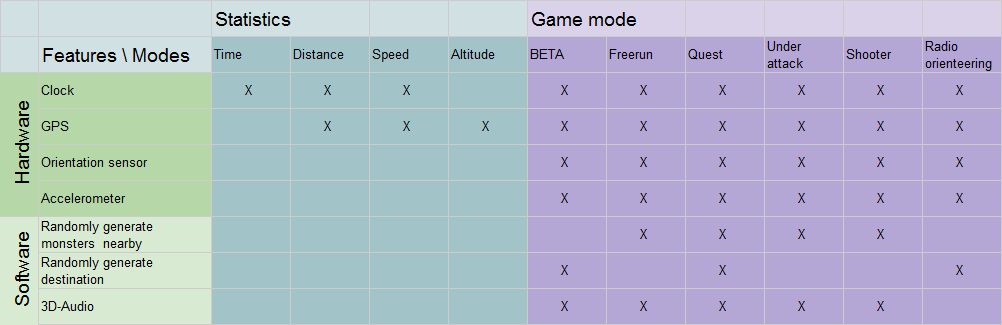
\includegraphics[width=1.1\textwidth]{\lyxdot \lyxdot /\lyxdot \lyxdot /\lyxdot \lyxdot /Dropbox/Chalmers/Kandidatarbete/tabbellfeatures}\caption{Scheme of what features are needed for different modes\label{fig:Scheme-of-features}}
\end{figure}


\item During the implementation of the game modes, a BETA-version will be
released. The BETA will then be evaluated usability wise by some test
persons. After getting feedback from the test group the app will be
updated accordingly to make sure that is is useable and fun to use.
\item Finally, if there is time, some advanced and further game functions
will be implemented:

\begin{itemize}
\item Multiplayer - Run together with a friend in the same game-world with
the same monsters and goals.
\item Some game mode including Geocaching%
\footnote{An outdoor ``Treasure hunt'' using GPS \citep{Groundspeak2014}.
\href{http://www.geocaching.com/}{http://www.geocaching.com/}%
} or Geocaching coordinates.
\end{itemize}
\end{enumerate}

\subsection{Plan B - Radio orienteering}

If the initial idea of a person running towards a directional sound
turns out to be a failure, the already written code will be used to
make an application to emulate radio orienteering - a sport where
the competitors have to find hidden controls by listening to a signal
caught up by a receiver carried by each contestant \citep{Radio-orienteringSverige2014}.

Instead of real controls and receivers, this application will rely
on generated GPS coordinartes and audio. By turning around with the
phone in hand, the audio level will change depending on if there’s
a control in the direction of which the phone is pointing. To clarify:
no panning will be involved - just the volume of the audio changing.

The GPS part of a radio orienteering application would work similar
to how it’d work in our initial application idea. The most drastic
change would be the audio not being panned, but instead relying completely
on the level of the sound always being in the centre - making it an
easier task to get working well. That would eliminate the problems
occurring when trying to make a sound appearing from a certain direction.


\section{Limitations}

Apart from being limited in time, one limitation is the ability for
the audio to be heard from the correct direction when the user is
standing still. It would be possible to use the gyroscope to calculate
the direction from which the sound is supposed to be heard from -
if the user is holding the phone in his/her hands, that is. If the
phone, however, is placed in the user’s pocket (or the like) the application
has to depend on how the user is approaching the goal destination,
using GPS technology.

When starting writing this report, possibilities to enhance the experience
with 3D positional audio was still being researched by members of
the group. There’s an API called OpenSL ES that claims to make it
easy to position audio binaurally (as well as processing it in other
ways) \citep*{KhronosGroup2014}. However, as for 2012, no actual
Android device seemed to support that specific feature \citep{Ratabouil2012}.
Neither did any of the project groups own phones. It turned out a
device had to implement a profile provided by OpenSL ES in order to
make use of all its functions.

Instead, if the sound is supposed to be heard from behind the user,
it will instead appear from one of the ears and gradually move towards
the center as the user is rotating towards the source. A voice or
sound informing the user that he/she is heading towards the wrong
direction might be a good alternative if the former turns out to be
difficult.

When developing the application, consideration that people might listen
to music when running, will be taken into account. Ideally for user
should be able to listen to music alongside using the application,
or possibly make the experience fun enough for the user not wanting
to listen to music while using the application.


\section{Method}

To begin with, information will be gathered about how to use the Android
APIs in the most efficient way for this kind of application. This
will include how to use activities, sensors and maps. Since we're
essentially developing an application to be run entirely on Android
platforms, this part of the research will be of huge importance for
the outcome.

Alongside with the coding-aspects mentioned above, information will
also be gathered on how specific areas (GPS, audio, etc.) work and
how they’re implemented using Java for Android. Most of the information
will probably come from e-books, as well as Android's developer pages
on the Internet.

When information is gathered the structure of the app will be decided.
Here UML-models will be drawn to make the structure clear. After the
modelling decisions are made sketches will be drawn to decide how
the GUI might look.

Then the coding process will start. The parts to be coded will be
the ones mentioned in the subsection Problem/Assignment. Alongside
with the coding testing will be made to make sure that everything
is working as expected. Where it is possible the tests will be made
as test cases, but it will also be important to test with real values,
as going out and running for real and see if it works.

An evaluation will be done when the first BETA-version is done. This
will be done by letting a test group use our app and evaluate it by
conducting an interview.


\subsection{Development}

The Scrum method will be used when developing the application - a
flexible Agile software development framework where the team works
more as a unit opposed to a traditional and sequential approach. The
division of labor will be decided in cycles (sprints). Each job occasion
will begin with a daily scrum - a short meeting where the group talks
about what’s going on, what’s about to happen as well as eventual
problems.

To handle the coding part of the development, Git will be used, which
is a version handling system that makes it easy to collaborate with
others in coding projects. It makes it possible for each team member
to work in the same classes and merge them when needed. Each specific
part of the application (audio, gps etc.) will be implemented in individual
branches.

When it comes to the testing part of the development, both the virtual
phone available in the Android developing environment will be used,
as well as our own phones. Testing is essential for our application
to run as smoothly as possible, so as many test cases as possible
will be covered.


\subsection{Literature studies}

The literature studies will partly involve how the human ear perceives
sound, and how it’s possible to imitate sounds coming from specific
directions using stereo headphones \citet{Roads1996}.

Literature about Android and how to best develop the app will also
be studied. This is necessary to make the app enjoyable for the user
and flexible enough to work on different kinds of phones. According
to the Android API Guide - Fragments , fragments seems like a good
way to decompose the functionality of an app into smaller parts (fragments)
that can be reusable and depending on the screen size show up in different
quantities.

Alongside the audio and Android studies, the sensors considering position
and orientation need to be studied. While GPS is the most natural
way to measure the position \citep{Sood2012}, there are various ways
to measure the user orientation. 

The orientation while in motion could be decided through the GPS bearing
\citep*{AndroidDevelopers2014}, which is calculated as the direction
the phone is travelling in. Although, while standing still and only
rotating on the spot, we might be able to use the magnetic field sensor
(compass) and accelerometer to provide an orientation of the phone
itself \citet{Sood2012}. This however has problems since the orientation
of the phone relative to the actual user is not always known (it dependa
on how the user is holding the phone).

Probably, as some initial testing shows, some combination of both
is preferable.


\section{Timetable}

In order to create preliminary time plan of the milestones and the
important phases of the project a Gantt chart was created. It is to
be found in \prettyref{fig:Gantt Chart}.

\begin{sidewaysfigure}
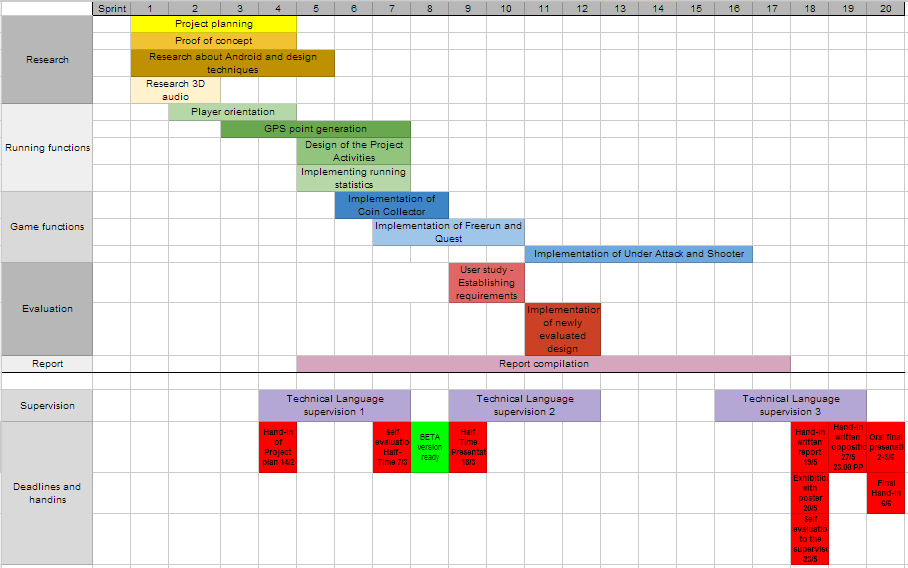
\includegraphics[width=0.9\paperwidth]{\lyxdot \lyxdot /\lyxdot \lyxdot /\lyxdot \lyxdot /Dropbox/Chalmers/Kandidatarbete/timetable}\caption{Preliminary Time Plan for the project \label{fig:Gantt Chart}}
\end{sidewaysfigure}


\pagebreak{}\bibliographystyle{apalike}
\phantomsection\addcontentsline{toc}{section}{\refname}\bibliography{References}

\end{document}
